% Exposición del paper «A Fast Wait-Free Solution to Read-Reclaim Races in Reference Counting» (Euro-Par 2024)
% Expositores: David (parte 1), Hugo (parte 2) y Diego (parte 3).
% Compilar: latexmk -pdf -interaction=nonstopmode -halt-on-error exposicion.tex
\documentclass[aspectratio=169,11pt]{beamer}
\usepackage[spanish,es-noshorthands,es-nodecimaldot,es-tabla]{babel}
\usepackage[T1]{fontenc}
\usepackage[sfdefault,lining]{FiraSans}
\usepackage[scale=0.86]{FiraMono}
\usepackage{booktabs,tabularx,array,graphicx,pifont,xcolor}
\usepackage{tikz}
\usetikzlibrary{arrows.meta,positioning,calc,babel}
\hypersetup{pdftitle={Exposición: A Fast Wait-Free Solution to Read-Reclaim Races in Reference Counting},pdfauthor={},pdfcreator={},pdfproducer={},pdfsubject={},pdfkeywords={}}

% ---------- paleta ----------
\definecolor{tinta}{HTML}{1B2430}
\definecolor{gris}{HTML}{5B6573}
\definecolor{acento}{HTML}{C8551F}   % el peso / talonario
\definecolor{hoja}{HTML}{1F5FA8}     % la hoja / contador
\definecolor{ok}{HTML}{1B7F3B}
\definecolor{mal}{HTML}{B3261E}
\definecolor{suave}{HTML}{EEF1F5}
\newcommand{\si}{\textcolor{ok}{\ding{51}}}
\newcommand{\no}{\textcolor{mal}{\ding{55}}}
\newcommand{\us}{\,\textmu s}
\newcommand{\clave}[1]{\textcolor{acento}{\textbf{#1}}}
\newcommand{\fuente}[1]{\par\vspace{2pt}{\scriptsize\color{gris}#1}}

% ---------- plantilla ----------
\setbeamertemplate{navigation symbols}{}
\setbeamercolor{normal text}{fg=tinta}
\setbeamercolor{structure}{fg=hoja}
\setbeamercolor{frametitle}{fg=tinta}
\setbeamerfont{frametitle}{size=\Large,series=\bfseries}
\setbeamertemplate{frametitle}{\vspace*{8pt}\insertframetitle\par\vspace{3pt}{\color{acento}\rule{1.6cm}{2.2pt}}\vspace*{-4pt}}
\setbeamertemplate{itemize item}{\textcolor{acento}{\small$\blacktriangleright$}}
\setbeamertemplate{itemize subitem}{\textcolor{gris}{--}}
\setbeamertemplate{enumerate item}{\textcolor{acento}{\bfseries\insertenumlabel.}}
\setbeamerfont{caption}{size=\scriptsize}
\newcommand{\elexpositor}{}
\newcommand{\expone}[1]{\renewcommand{\elexpositor}{#1}}
\setbeamertemplate{footline}{\leavevmode\hbox to\paperwidth{\hspace{10pt}\color{gris}\scriptsize%
  \ifx\elexpositor\empty\else Expone: \textbf{\textcolor{tinta}{\elexpositor}}\quad·\quad\fi
  de Wolff, Anderson, Keller y Seletskiy · Euro-Par 2024\hfill\insertframenumber\,/\,\inserttotalframenumber\hspace{10pt}}\vspace{6pt}}
\newcommand{\divisor}[4]{{\setbeamertemplate{footline}{}\begin{frame}[plain]
  \vfill{\color{acento}\large\bfseries Parte #1}\par\medskip{\fontsize{30}{34}\selectfont\bfseries #2}\par\bigskip
  {\large Expone: \textbf{#3}}\par\medskip{\color{gris}#4}\vfill\end{frame}}}
\setlength{\tabcolsep}{5pt}

\title{A Fast Wait-Free Solution to Read-Reclaim Races in Reference Counting}
\subtitle{Conteo de referencias concurrente: sin candados, sin esperas y sin memoria extra}
\date{}

\begin{document}

% =====================================================================
{\setbeamertemplate{footline}{}
\begin{frame}[plain]
  \vspace*{6mm}
  {\color{acento}\small\bfseries EXPOSICIÓN DE PAPER}\par\smallskip
  {\fontsize{24}{28}\selectfont\bfseries A Fast Wait-Free Solution to\\ Read-Reclaim Races in Reference Counting\par}
  \medskip
  {\large\color{gris}Conteo de referencias concurrente: sin candados, sin esperas y sin memoria extra\par}
  \vfill
  \begin{columns}[T]
    \column{0.58\textwidth}
    {\small\color{gris}Paper}\\
    Ivo Gabe de Wolff, Daniel Anderson, Gabriele K. Keller y Aleksei Seletskiy\\
    {\small Universidad de Utrecht · Carnegie Mellon University}\\
    {\small Euro-Par 2024 · LNCS 14803 · págs. 103–118 · doi 10.1007/978-3-031-69583-4\_8}
    \column{0.36\textwidth}
    {\small\color{gris}Expositores}\\[2pt]
    {\large\bfseries David · Hugo · Diego}
  \end{columns}
  \vspace*{4mm}
\end{frame}}

\begin{frame}{Plan de la exposición}
  \renewcommand{\arraystretch}{1.2}\small
  \begin{tabularx}{\linewidth}{@{}l l X r@{}}
    \toprule
    & \textbf{Expone} & \textbf{Contenido} & \textbf{Tiempo}\\
    \midrule
    1 & \textbf{David} & El problema: conteo de referencias, la carrera \emph{read-reclaim}, garantías de progreso, lo que había y qué aporta el paper. \emph{Demo: la carrera con AddressSanitizer.} & $\approx$ 10 min\\
    2 & \textbf{Hugo} & La solución: conteo ponderado, algoritmo 1 (\texttt{store}/\texttt{load}), empaquetado en 64 bits, la recarga \emph{wait-free} (algoritmo 2) y un ejemplo con números. \emph{Demo: el simulador encuentra los fallos.} & $\approx$ 10 min\\
    3 & \textbf{Diego} & Corrección y evaluación: demostración, coste, extensiones, experimentos del paper, \emph{nuestras pruebas en local}, crítica y conclusiones. & $\approx$ 10 min\\
    \bottomrule
  \end{tabularx}
  \vfill
  {\footnotesize\color{gris}Pruebas en local: Intel i5-10400 (12 hilos), WSL Ubuntu 24.04, g++ 13.3, código original de los autores.}
\end{frame}

\begin{frame}{Una analogía para toda la exposición}
  \renewcommand{\arraystretch}{1.1}\small
  \begin{tabularx}{\linewidth}{@{}>{\bfseries}p{4.2cm} p{4.6cm} X@{}}
    \toprule
    Analogía & Término del paper & Qué es de verdad\\
    \midrule
    Libro & objeto & datos en el montón\\
    \textcolor{hoja}{Hoja} de usuarios & \emph{reference count} (rc) & contador junto al objeto\\
    Pase en tu mano & \emph{shared pointer} (peso 1) & referencia propia e inmutable\\
    \textcolor{acento}{Cartel} en la pared & \emph{atomic shared pointer} & variable compartida y mutable\\
    \textcolor{acento}{Talonario} del cartel & \emph{weight} (peso) & bits altos del puntero\\
    Bibliotecario / lector & \texttt{store} / \texttt{load} & escritor / lector\\
    Tirar el libro & \emph{reclaim} & liberar la memoria\\
    \bottomrule
  \end{tabularx}
  \vfill
  \begin{center}\small La idea del paper: \clave{el cartel lleva un talonario de tickets ya apuntados en la hoja}. Leer = arrancar un ticket.\end{center}
\end{frame}

% =====================================================================
\expone{David}
\divisor{1}{El problema}{David}{Conteo de referencias · la carrera \emph{read-reclaim} · lo que había}

\begin{frame}{El paper en una frase}
  \begin{block}{}
    \large ¿Cómo leer un puntero compartido a un objeto con conteo de referencias \textbf{mientras otro hilo lo cambia}, sin candados, sin que nadie espere y sin gastar memoria extra?
  \end{block}
  \bigskip
  \begin{columns}[T]
    \column{0.5\textwidth}
    \begin{itemize}
      \item Euro-Par 2024 (LNCS 14803), Madrid.
      \item Utrecht (de Wolff, Keller) y CMU (Anderson, Seletskiy).
      \item Sello \emph{Artifact Evaluated}: código y \emph{benchmarks} públicos (Zenodo y GitHub).
    \end{itemize}
    \column{0.46\textwidth}
    \begin{itemize}
      \item Mejora la técnica \emph{split reference count}, que se usa en producción (Folly, de Facebook) pero solo es \emph{lock-free}.
      \item La hace \textbf{\emph{wait-free}} y la explica de forma más sencilla.
    \end{itemize}
  \end{columns}
\end{frame}

\begin{frame}[fragile]{Conteo de referencias en 30 segundos}
  \begin{columns}[T]
    \column{0.52\textwidth}
\begin{semiverbatim}\small
auto a = std::make_shared<Libro>(); // rc = 1
\{
    auto b = a;      // copia:       rc = 2
\}                    // b se destruye: rc = 1
a = nullptr;         // rc = 0: se libera
\end{semiverbatim}
    \smallskip
    {\small Se usa en \texttt{std::shared\_ptr} (C++), \texttt{Arc} (Rust), Swift, CPython.}
    \column{0.44\textwidth}
    \begin{itemize}
      \item Copiar una referencia: \textbf{rc += 1}. Destruirla: \textbf{rc $-$= 1}.
      \item rc llega a 0 $\Rightarrow$ se libera \textbf{en ese momento}.
      \item Ventaja: si rc = 1, el dueño único puede \textbf{modificar en el sitio}.
      \item Problemas clásicos: ciclos (punteros débiles) y \clave{concurrencia} — el tema del paper.
    \end{itemize}
  \end{columns}
\end{frame}

\begin{frame}[fragile]{\emph{Shared pointer} y \emph{atomic shared pointer}}
  \begin{columns}[T]
    \column{0.5\textwidth}
    \begin{itemize}
      \item \textbf{Shared pointer}: puntero \emph{inmutable} con conteo. Su contador ya es seguro con hilos.
      \item \textbf{Atomic shared pointer}: celda \emph{mutable} que contiene un shared pointer; varios hilos la leen (\texttt{load}) y la cambian (\texttt{store}). En C++20: \texttt{std::atomic<std::shared\_ptr<T>{}>}.
    \end{itemize}
\begin{semiverbatim}\scriptsize
std::atomic<std::shared_ptr<Config>> config;
auto c = config.load();   // lector: su pase
config.store(std::make_shared<Config>(n));
\end{semiverbatim}
    \column{0.48\textwidth}
    \centering\includegraphics[width=\linewidth]{figuras/paper_fig1.pdf}
    \fuente{Fig. 1 del paper: dónde se guarda el contador. El algoritmo se explica con (a); (b) es igual con una indirección; (c) \emph{aliasing}, en la sección 5.2.}
  \end{columns}
\end{frame}

\begin{frame}{La carrera \emph{read-reclaim}}
  \centering
  \begin{tikzpicture}[x=3.25cm,y=1cm,paso/.style={draw,rounded corners=3pt,fill=white,align=center,font=\small,minimum height=9mm,text width=3.1cm}]
    \node[font=\bfseries,text=hoja,anchor=east] at (-0.15,1.2) {Ana (lee)};
    \node[font=\bfseries,text=acento,anchor=east] at (-0.15,-0.4) {Beto (escribe)};
    \node[paso,draw=hoja] (a1) at (0.55,1.2) {1. lee el cartel: \textbf{A}};
    \node[paso,draw=gris,dashed,text=gris] (ap) at (1.75,1.2) {\itshape el sistema la pausa};
    \node[paso,draw=acento] (b2) at (1.75,-0.4) {2. pone \textbf{B} en el cartel};
    \node[paso,draw=acento] (b3) at (2.95,-0.4) {3. rc(A) $-$= 1 $\to$ 0\\ \textbf{libera A}};
    \node[paso,draw=mal,fill=mal!8] (a4) at (2.95,1.2) {4. rc(A) += 1 \textcolor{mal}{\ding{55}}\\ \emph{use-after-free}};
    \draw[-Latex,thick,hoja] (a1) -- (ap); \draw[-Latex,thick,hoja] (ap) -- (a4);
    \draw[-Latex,thick,acento] (b2) -- (b3);
    \draw[-Latex,gris] (0.05,-1.3) -- node[below,font=\scriptsize]{tiempo} (3.6,-1.3);
  \end{tikzpicture}
  \bigskip
  \begin{itemize}
    \item Leer el puntero y apuntarse en el contador son \clave{dos pasos}; entre ellos, otro hilo puede liberar el objeto.
    \item La ventana dura nanosegundos: el fallo es rarísimo, pasa las pruebas y aparece en producción. Es una causa típica de vulnerabilidades.
  \end{itemize}
\end{frame}

\begin{frame}{¿Por qué no hacerlo en un solo paso?}
  \begin{columns}[c]
    \column{0.47\textwidth}
    \centering
    \begin{tikzpicture}[caja/.style={draw,thick,rounded corners=4pt,align=center,font=\small,inner sep=6pt}]
      \node[caja,draw=acento,fill=acento!8] (c) {\textbf{cartel}\\ variable compartida\\ \texttt{0x5000}};
      \node[caja,draw=hoja,fill=hoja!8,below=1.3cm of c] (l) {\textbf{libro A}\\ rc (hoja) = 1 · datos\\ \texttt{0x7F3A\dots}};
      \draw[-Latex,thick] (c) -- node[right,font=\scriptsize]{apunta a} (l);
    \end{tikzpicture}
    \par\smallskip{\small Puntero y contador viven en \textbf{dos sitios distintos} de la memoria.}
    \column{0.5\textwidth}
    \renewcommand{\arraystretch}{1.2}\footnotesize
    \begin{tabular}{@{}p{4.6cm}c@{}}
      \toprule
      Instrucción atómica & ¿Existe hoy?\\
      \midrule
      \texttt{fetch\_and\_add}, \texttt{swap}, CAS (64 bits) & \si\\
      CAS doble anchura (2 palabras \emph{contiguas}) & \si\\
      DCAS (2 palabras \emph{separadas}) & \no\\
      \texttt{fetch\_and\_add} de 128 bits & \no\\
      \bottomrule
    \end{tabular}
    \par\medskip
    Una instrucción atómica abarca \clave{una palabra}: no puede leer el cartel y modificar la hoja a la vez.
  \end{columns}
\end{frame}

\begin{frame}{Garantías de progreso}
  \renewcommand{\arraystretch}{1.2}\small
  \begin{tabularx}{\linewidth}{@{}l X X@{}}
    \toprule
    \textbf{Garantía} & \textbf{Definición (Herlihy, 1991)} & \textbf{Ejemplo: sumar 1 a un contador}\\
    \midrule
    Bloqueante & un hilo puede esperar indefinidamente a otro & protegerlo con un candado\\
    \emph{Lock-free} & en todo momento \textbf{algún} hilo termina en un número finito de pasos & bucle CAS: si mi CAS falla es porque otro tuvo éxito, pero yo podría fallar siempre\\
    \emph{Wait-free} & \textbf{cada} hilo termina en un número \textbf{acotado} de sus propios pasos & \texttt{fetch\_and\_add}: una instrucción, pase lo que pase\\
    \bottomrule
  \end{tabularx}
  \vfill
  \small\textbf{¿Por qué exigir \emph{wait-free} aquí?} La gestión de memoria está en todas partes: si una lectura de un puntero compartido puede atascarse, cualquier parte del programa puede atascarse. \emph{Wait-free} da un tiempo máximo garantizado y latencias predecibles.
\end{frame}

\begin{frame}{Lo que había}
  \renewcommand{\arraystretch}{1.1}\footnotesize
  \begin{tabularx}{\linewidth}{@{}p{5.5cm} c c c X@{}}
    \toprule
    Solución & \emph{Wait-free} & Sin mem. extra & Hw. actual & Precio\\
    \midrule
    Candado (\texttt{std::atomic<shared\_ptr>} de GCC) & \no & \si & \si & bloqueante\\
    Valois; Michael y Scott (1995) & \no & \no & \si & gestor propio\\
    Detlefs, Martin, Moir y Steele (2001) & \no & \si & \no & necesita DCAS\\
    Herlihy et al. (2005); Gidenstam et al. (2009) & \no & \no & \si & reclamación diferida\\
    Sundell (2005) & \si & \si & \si & cada CAS cuesta $\Theta(P)$\\
    Anderson, Blelloch y Wei, CDRC (2021–22) & --- & \no & \si & reclamación diferida\\
    \emph{Split reference count} (Williams, Folly) & \no & \si & \si & \emph{lock-free}\\
    \midrule
    \textbf{Este paper} & \si & \si & \si & CAS: \emph{lock-free}\\
    \bottomrule
  \end{tabularx}
  \vfill
  \small Exigencias: que funcione, que nadie espere, que no gaste memoria y que sea rápido. Ninguna solución anterior cumplía las cuatro.
\end{frame}

\begin{frame}{Contribuciones}
  \begin{enumerate}
    \item Un \emph{atomic shared pointer} \clave{wait-free} para \texttt{load}, \texttt{store} y \texttt{swap}, sin reclamación diferida y sin memoria extra.
    \item \texttt{store} en tiempo constante; \texttt{load} casi siempre \textbf{una instrucción atómica} y, en el peor caso, $O(P)$ con $P$ = hilos que usan esa variable.
    \item \emph{Compare-and-swap} y punteros \emph{aliased}: también soportados, pero solo \emph{lock-free}.
    \item Reexplica el \emph{split reference count} como un caso de \textbf{conteo de referencias ponderado}: una explicación (y una demostración) más sencilla.
    \item Experimentos: el más rápido de los que no gastan memoria extra y la menor latencia de lectura.
  \end{enumerate}
\end{frame}

\begin{frame}{Demo 1: la carrera existe (AddressSanitizer)}
  \centering
  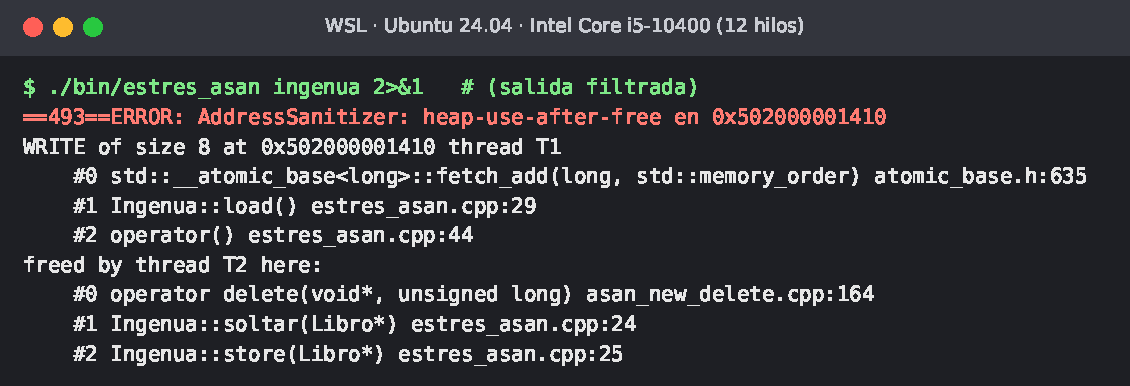
\includegraphics[width=0.98\linewidth,height=0.5\textheight,keepaspectratio]{graficos/captura_asan_ingenua.pdf}\par\smallskip
  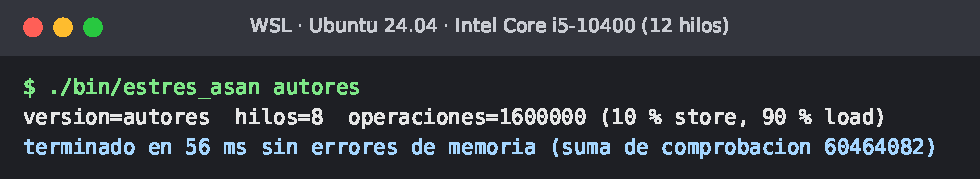
\includegraphics[width=0.7\linewidth,height=0.17\textheight,keepaspectratio]{graficos/captura_asan_autores.pdf}
  \fuente{8 hilos, 10 \% store / 90 \% load en la misma celda. Arriba: versión ingenua. Abajo: código de los autores.}
\end{frame}

\begin{frame}{La idea, antes de pasar a Hugo}
  \centering
  \begin{tikzpicture}[caja/.style={draw,thick,rounded corners=4pt,align=center,inner sep=7pt}]
    \node[caja,draw=acento,fill=acento!8] (c) {\textbf{Cartel}\\ libro A · talonario \textbf{104}};
    \node[caja,draw=hoja,fill=hoja!8,right=3.2cm of c] (l) {\textbf{Libro A}\\ hoja = \textbf{106} = 104 + 1 + 1};
    \draw[-Latex,thick] (c) -- (l);
    \node[caja,draw=gris,below=1.1cm of c,font=\small] (ana) {pase de Ana (1)};
    \node[caja,draw=gris,right=0.4cm of ana,font=\small] (beto) {pase de Beto (1)};
    \draw[-Latex,gris] (ana) -- (l); \draw[-Latex,gris] (beto) -- (l);
  \end{tikzpicture}
  \bigskip
  \begin{itemize}
    \item Los tickets del talonario \textbf{ya están apuntados} en la hoja del libro: son referencias pagadas por adelantado.
    \item Leer = \clave{arrancar un ticket} con un \texttt{fetch\_and\_add}, que a la vez dice qué libro hay. La hoja no se toca.
    \item Leer y apuntarse pasan a ser \textbf{un solo paso}: la ventana peligrosa desaparece.
  \end{itemize}
\end{frame}

% =====================================================================
\expone{Hugo}
\divisor{2}{La solución}{Hugo}{Conteo ponderado · algoritmo 1 · empaquetado · recarga \emph{wait-free}}

\begin{frame}{Conteo de referencias ponderado (Bevan; Watson y Watson, 1987)}
  \begin{columns}[T]
    \column{0.47\textwidth}
    \begin{itemize}\small
      \item Cada referencia tiene un \textbf{peso}; el contador es la \textbf{suma de pesos}.
      \item Soltar: restar su peso.
      \item \textbf{Clonar}: repartir el peso, \clave{sin tocar el contador}.
      \item Clonar una de peso 1 exige subir antes su peso.
    \end{itemize}
    \column{0.5\textwidth}
    \renewcommand{\arraystretch}{1.2}\small
    \begin{tabular}{@{}llcc@{}}
      \toprule
      Acción & Pesos & Hoja & ¿Toca la hoja?\\
      \midrule
      inicio & X = 10 & 10 & ---\\
      clonar X en Y & X = 6, Y = 4 & 10 & \textbf{no}\\
      tirar Y & X = 6 & 6 & sí ($-4$)\\
      clonar X en Z & X = 3, Z = 3 & 6 & \textbf{no}\\
      tirar Z y X & --- & 0 & libera\\
      \bottomrule
    \end{tabular}
    \par\medskip
    En memoria compartida, «tocar la hoja» es tocar una posición lejana: evitarlo es lo que \clave{elimina la carrera}.
  \end{columns}
\end{frame}

\begin{frame}{El peso en el \emph{atomic shared pointer}}
  \centering\includegraphics[width=0.7\linewidth]{figuras/paper_fig2.pdf}
  \fuente{Fig. 2 del paper. (a) 104 + 1 + 1 = 106. (b) Tras un \texttt{load}: el cartel baja a 103, aparece un pase nuevo y la hoja sigue en 106.}
  \medskip
  \begin{itemize}\small
    \item Al crear el cartel se le da un peso $C \gg P$ y se suma $C$ a la hoja. Cada pase pesa 1.
    \item Invariante: \textbf{hoja $\ge$ peso del cartel + pases}; igual cuando no hay operaciones a medias. Por arriba es seguro; por abajo, liberaríamos con lectores dentro.
  \end{itemize}
\end{frame}

\begin{frame}{Algoritmo 1: \texttt{store} y \texttt{load}}
  \centering\includegraphics[width=0.72\linewidth,height=0.36\textheight,keepaspectratio]{figuras/paper_alg1.pdf}
  \fuente{Algoritmo 1 del paper.}
  \begin{columns}[T]
    \column{0.48\textwidth}\footnotesize
    \textbf{\texttt{store}}
    \begin{enumerate}
      \item sumar $C$ al objeto nuevo \textbf{antes} de publicarlo;
      \item \texttt{swap}: poner (nuevo, $C$) y llevarse (viejo, $w$) de golpe;
      \item restar al viejo \textbf{solo} el sobrante $w$.
    \end{enumerate}
    \column{0.48\textwidth}\footnotesize
    \textbf{\texttt{load}}
    \begin{enumerate}
      \item \texttt{fetch\_and\_add}($-$\texttt{pack(null,1)}): un ticket menos y el valor anterior, en \clave{una instrucción};
      \item si quedan menos de $P$: recargar (algoritmo 2);
      \item devolver un pase de peso 1, ya pagado.
    \end{enumerate}
  \end{columns}
\end{frame}

\begin{frame}{Por qué desaparece la carrera}
  {\small Cartel (A, 5), hoja de A = 5. Ana: \texttt{load} = un \texttt{fetch\_and\_add} (F). Beto: \texttt{store(B)} = sumar $C$ a B (S1), \texttt{swap} (S2), restar sobrante a A (S3). F y S2 tocan \textbf{la misma palabra}: el procesador los ordena.}
  \medskip
  \begin{columns}[T]
    \column{0.48\textwidth}
    \begin{block}{Caso 1: F antes que S2}
      \small Ana arranca un ticket: cartel (A, 4), Ana tiene un pase de A.\\
      S2 recoge (A, 4); S3 resta 4: hoja de A = 5 $-$ 4 = \textbf{1} = el pase de Ana.\\
      A vive mientras Ana lo usa y se libera cuando lo suelta.
    \end{block}
    \column{0.48\textwidth}
    \begin{block}{Caso 2: F después de S2}
      \small El cartel ya muestra (B, $C$): Ana se lleva un pase de \textbf{B}, respaldado desde S1.\\
      S3 resta 5 a A: se libera sin nadie dentro.\\
      Ana nunca toca A.
    \end{block}
  \end{columns}
  \bigskip
  \centering\clave{No hay tercer caso}: el estado «he leído pero no me he apuntado» ya no existe.
\end{frame}

\begin{frame}{Empaquetar puntero y peso en 64 bits}
  \begin{columns}[c]
    \column{0.42\textwidth}
    \centering\includegraphics[width=\linewidth]{figuras/paper_fig3.pdf}
    \fuente{Fig. 3 del paper.}
    \column{0.55\textwidth}
    \begin{itemize}\small
      \item x86-64 usa 48 bits de dirección: \textbf{16 bits altos libres} para el peso ($C \le 2^{16}-1$); con los 3 bits de alineación, 19 ($C \le 2^{19}-1$).
      \item Restar un ticket = restar $2^{48}$ a la palabra entera:
    \end{itemize}
    {\ttfamily\small\quad\ \ 0x\textcolor{acento}{0068}\,7F3A12345670\\
    \quad $-$ 0x\textcolor{acento}{0001}\,000000000000\\
    \quad = 0x\textcolor{acento}{0067}\,7F3A12345670}
    \begin{itemize}\small
      \item La dirección no cambia; el acarreo sale por arriba. Con \texttt{null}, el peso da la vuelta sin estropear el puntero.
      \item El contador del objeto, de 64 bits: con 32 bits y $C = 2^{19}$, bastarían 8192 carteles para desbordarlo.
    \end{itemize}
  \end{columns}
\end{frame}

\begin{frame}{Recargar el talonario: el punto delicado}
  \begin{columns}[T]
    \column{0.5\textwidth}
    Cuando un \texttt{load} deja el peso por debajo de $P$, \textbf{ese hilo} recarga: reserva $C-w$ en la hoja y sube el peso lo mismo. Dos trampas:
    \begin{itemize}\small
      \item el cartel pudo cambiar de libro (\texttt{store} intermedio);
      \item otro hilo pudo recargar ya (desbordamiento).
    \end{itemize}
    $\Rightarrow$ no vale \texttt{fetch\_and\_add}: hace falta un \textbf{CAS} («solo si sigue como lo vi»).
    \column{0.46\textwidth}
    \begin{block}{Requisitos para ser \emph{wait-free}}
      \textbf{R-1}: $C \ge 2P$.\\[3pt]
      \textbf{R-2}: el peso solo \textbf{baja de 1 en 1} o se \textbf{fija por encima de $P$}.
    \end{block}
    \small Con R-1, tras recargar:\\ $\text{actual} + C - w \ \ge\ 0 + 2P - (P-1) = P+1 > P$.\\[3pt]
    Consecuencia de R-2: si el CAS falla y el peso \textbf{subió}, alguien ya recargó $\Rightarrow$ \clave{salida temprana}.
  \end{columns}
\end{frame}

\begin{frame}{La idea informal: Figura 4}
  \begin{columns}[c]
    \column{0.45\textwidth}
    \centering\includegraphics[width=\linewidth]{figuras/paper_fig4.pdf}
    \fuente{Fig. 4 del paper: peso de un cartel en el tiempo; la línea es $P$.}
    \column{0.52\textwidth}\small
    \begin{enumerate}
      \item[1] Un hilo empieza un \texttt{load} con el peso bajo: va a recargar.
      \item[2] Otro hilo recarga antes: el peso salta por encima de $P$.
      \item[3] El CAS del primero falla. El peso vuelve a ser bajo, pero \textbf{mayor que el que vio}: por R-2, alguien lo subió por encima de $P$. Puede irse.
      \item[4] Quienes lo bajaron después de 2 completan la siguiente recarga.
    \end{enumerate}
    \medskip
    \clave{Quien mete el talonario en la zona roja, lo saca}; si otro se adelanta, se va.
  \end{columns}
\end{frame}

\begin{frame}{Algoritmo 2: \texttt{increase\_weight}}
  \centering\includegraphics[width=0.72\linewidth,height=0.3\textheight,keepaspectratio]{figuras/paper_alg2.pdf}
  \fuente{Algoritmo 2 del paper.}
  \begin{columns}[T]
    \column{0.52\textwidth}\footnotesize
    \begin{enumerate}
      \item reservar $C - w$ en la hoja \textbf{antes} del CAS;
      \item CAS: si el cartel sigue en (ptr, actual), sumar $C - w$;
      \item éxito: terminar;
      \item otro puntero o \textbf{peso mayor}: devolver la reserva y salir;
      \item peso menor: reintentar con el nuevo valor.
    \end{enumerate}
    \column{0.44\textwidth}\footnotesize
    Los pesos esperados forman una cadena \textbf{estrictamente decreciente} entre $P-1$ y 0: \clave{como mucho $P$ intentos}.
  \end{columns}
\end{frame}

\begin{frame}{Ejemplo completo: $P = 4$, $C = 8$}
  \renewcommand{\arraystretch}{1.0}\footnotesize
  \begin{tabularx}{\linewidth}{@{}r X c c c c c@{}}
    \toprule
    Paso & Qué pasa & Tickets & Hoja & Pases & $O$ & $P-|O|$\\
    \midrule
    1 & \texttt{store}: cartel con 8, hoja con 8 & 8 & 8 & 0 & $\emptyset$ & 4\\
    2 & cuatro lecturas normales (8 $\to$ 4) & 4 & 8 & 4 & $\emptyset$ & 4\\
    3 & Ana lee 4 $\to$ 3: \textbf{ofensa}; recargará con $w = 3$ & 3 & 8 & 5 & \{Ana\} & 3\\
    4 & Beto lee 3 $\to$ 2: ofensa; recargará con $w = 2$ & 2 & 8 & 6 & \{Ana, Beto\} & 2\\
    5–6 & Ana reserva 5; Beto reserva 6 & 2 & 19 & 6 & \{Ana, Beto\} & 2\\
    7 & Ana: CAS(3 $\to$ 8) falla; ve 2 < 3 $\to$ reintenta & 2 & 19 & 6 & \{Ana, Beto\} & 2\\
    8 & Ana: CAS(2 $\to$ 7) éxito; $O$ se vacía & 7 & 19 & 6 & $\emptyset$ & 4\\
    9 & Beto: CAS(2 $\to$ 8) falla; ve 7 > 2 $\to$ \textbf{sale} & 7 & 19 & 6 & $\emptyset$ & 4\\
    10 & Beto devuelve su reserva de 6 & 7 & \textbf{13} & 6 & $\emptyset$ & 4\\
    \bottomrule
  \end{tabularx}
  \fuente{Al final: 7 tickets + 6 pases = 13 = hoja. La hoja nunca va por debajo.}
\end{frame}

\begin{frame}{Demo 2 (1/2): un simulador encuentra los fallos de cada variante}
  \centering
  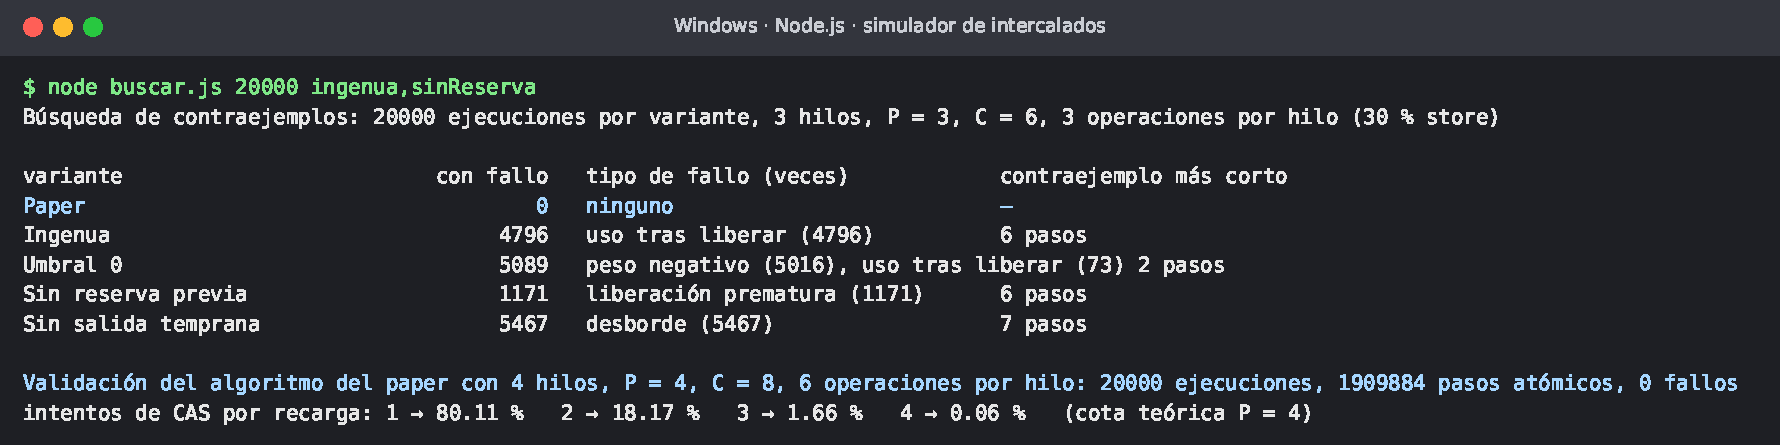
\includegraphics[width=0.98\linewidth,height=0.7\textheight,keepaspectratio]{graficos/captura_simulador.pdf}
  \fuente{Simulador de intercalados (paso atómico a paso atómico) que comprueba los invariantes tras cada paso. Paper: 0 fallos; cada variante rota falla en 2 a 7 pasos.}
\end{frame}

\begin{frame}{Demo 2 (2/2): traza de un contraejemplo}
  \centering
  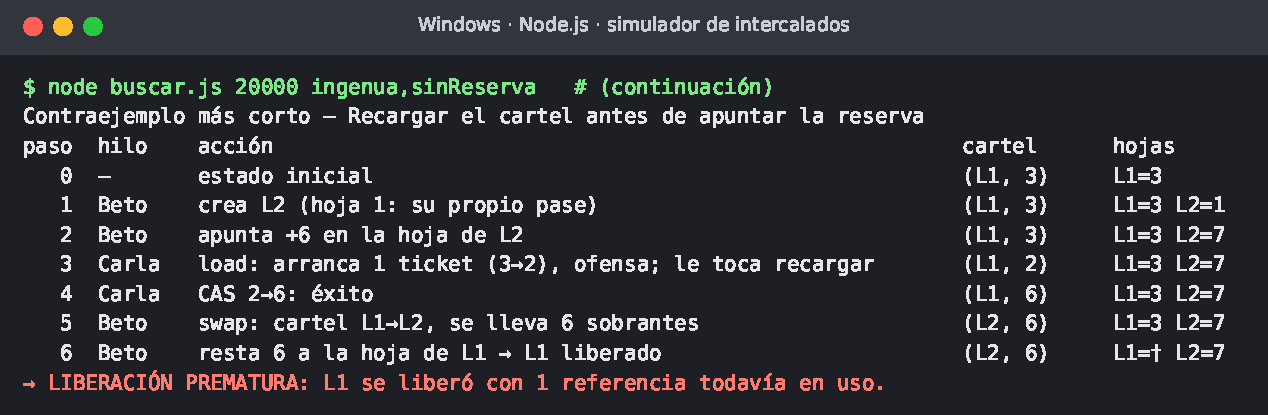
\includegraphics[width=0.98\linewidth,height=0.72\textheight,keepaspectratio]{graficos/captura_simulador_traza.pdf}
  \fuente{Intercalado mínimo que rompe una variante, con el estado tras cada paso atómico.}
\end{frame}

% =====================================================================
\expone{Diego}
\divisor{3}{Corrección y evaluación}{Diego}{Demostración · coste · extensiones · experimentos · pruebas en local}

\begin{frame}{La demostración: el peso nunca es negativo}
  \begin{columns}[T]
    \column{0.5\textwidth}
    \small
    \textbf{Por qué importa}: el peso está en 16 bits sin signo; $-1$ sería 65\,535 \emph{tickets fantasma} sin respaldo $\Rightarrow$ \emph{use-after-free}.\par\medskip
    \textbf{Ofensa}: decrementar el peso cuando vale $\le P$.\\
    \textbf{$O$}: multiconjunto de ofensores; se vacía cuando alguien fija el peso por encima de $P$.
    \column{0.47\textwidth}
    \small
    \textbf{Invariante 1}: cada hilo está en $O$ como mucho una vez (quien ofende recarga, y no sale sin que $O$ se vacíe).\par\medskip
    \textbf{Invariante 2}: peso $\ge P - |O|$ (desde el último vaciado solo baja de 1 en 1; cada bajada en zona roja suma 1 a $|O|$).
  \end{columns}
  \bigskip
  \begin{block}{}
    \centering\large peso $\ \ge\ P - |O|\ \ge\ P - P\ =\ 0$
  \end{block}
  \small Por eso el umbral de recarga es $P$ y no 0: es el colchón para que todos ofendan una vez a la vez.
\end{frame}

\begin{frame}{Coste}
  \begin{columns}[T]
    \column{0.48\textwidth}
    \begin{itemize}\small
      \item El bucle CAS solo repite si \textbf{otro} hilo bajó el peso: la cadena $w_0 > w_1 > \dots \ge 0$, con $w_0 \le P-1$, tiene como mucho $P$ elementos.
      \item Peor caso de \texttt{load}: $O(P)$, con $P$ = hilos que \textbf{usan esa variable}.
      \item Amortizado: tras recargar quedan $\approx C$ tickets; con $C = 2^{19}$ y $P = 2^{16}$ hay $\approx$ 458\,752 lecturas entre recargas (2 por millón).
    \end{itemize}
    \column{0.48\textwidth}
    \renewcommand{\arraystretch}{1.1}\footnotesize
    \begin{tabular}{@{}lll@{}}
      \toprule
      Operación & Coste & Garantía\\
      \midrule
      \texttt{store}, \texttt{swap} & $O(1)$ & \emph{wait-free}\\
      \texttt{load} & 1 instr.; $O(P)$ peor & \emph{wait-free}\\
      compare-and-swap & sin cota & \emph{lock-free}\\
      \texttt{load} \emph{aliased} & sin cota & \emph{lock-free}\\
      \bottomrule
    \end{tabular}
  \end{columns}
\end{frame}

\begin{frame}{Extensiones (sección 5)}
  \begin{columns}[T]
    \column{0.45\textwidth}\footnotesize
    \begin{itemize}
      \item \textbf{\texttt{null}}: con el peso en los bits altos, restar tickets a \texttt{null} solo da la vuelta al peso; no hace falta recargar.
      \item \textbf{Punteros débiles}: ortogonales; misma técnica.
      \item \textbf{Compare-and-set}: bucle CAS sobre la palabra (libro, tickets). Cualquier lectura cambia los tickets y hace fallar al escritor $\Rightarrow$ solo \emph{lock-free}.
      \item \textbf{\emph{Aliasing}}: dos punteros en 128 bits; camino rápido con \texttt{fetch\_and\_add} en los primeros 64 y, si hay \emph{aliasing}, bucle CAS de 128 bits (\emph{lock-free}).
    \end{itemize}
    \column{0.53\textwidth}
    \includegraphics[width=\linewidth]{figuras/paper_alg3.pdf}
    \fuente{Algoritmo 3 del paper.}
  \end{columns}
\end{frame}

\begin{frame}{Experimentos del paper: montaje}
  \begin{columns}[T]
    \column{0.5\textwidth}\small
    \begin{itemize}
      \item $C = 2^{19}$, $P = 2^{16}$ (R-1 con holgura).
      \item Rendimiento: 4× Xeon E7-8867, 72 núcleos, 144 hilos.
      \item Latencia: Xeon w7-3465X, 28 núcleos, 56 hilos.
      \item \textbf{Pila concurrente}: $n$ pilas, $u$\,\% de actualizaciones (sacar de una pila y meter en otra con \emph{compare-and-set}); el resto lee la cima (\texttt{load}).
    \end{itemize}
    \column{0.46\textwidth}
    \renewcommand{\arraystretch}{1.1}\footnotesize
    \begin{tabular}{@{}ll@{}}
      \toprule
      Rival & Estrategia\\
      \midrule
      Libstdc++ (GCC) & candados\\
      Williams & \emph{split refcount}\\
      Folly (Facebook) & \emph{split refcount}\\
      Anderson & \emph{hazard pointers}\\
      \bottomrule
    \end{tabular}
  \end{columns}
\end{frame}

\begin{frame}{Figura 5: rendimiento}
  \begin{columns}[c]
    \column{0.6\textwidth}
    \includegraphics[width=\linewidth]{figuras/paper_fig5.pdf}
    \fuente{Fig. 5 del paper: millones de operaciones por segundo frente a hilos; la línea discontinua marca 144.}
    \column{0.38\textwidth}\small
    \begin{itemize}
      \item Con 1 hilo, \textbf{Our} es la más rápida en todos los paneles.
      \item Gana siempre a los rivales sin memoria extra (GCC, Williams, Folly): con 1 pila y 144 hilos, $\approx$7× Williams y $\approx$20× Folly.
      \item Frente a Anderson depende de la \textbf{contención}: gana con $n = 10, u = 1$ y con $10^6$ pilas; pierde con una sola pila (las actualizaciones usan el CAS \emph{lock-free}).
    \end{itemize}
  \end{columns}
\end{frame}

\begin{frame}{Figura 6: latencia}
  \begin{columns}[c]
    \column{0.6\textwidth}
    \includegraphics[width=\linewidth]{figuras/paper_fig6.pdf}
    \fuente{Fig. 6 del paper: percentiles 25, 50 y 75 (caja) y 1 y 99 (bigotes); con $p = 56$, escala logarítmica.}
    \column{0.38\textwidth}\small
    \renewcommand{\arraystretch}{1.12}
    \begin{tabular}{@{}lr@{}}
      \toprule
      \texttt{load}, $p = 56$ & mediana\\
      \midrule
      \textbf{Ours} & \textbf{1,14\us}\\
      Anderson & 2,58\us\\
      Folly & 11,6\us\\
      Libstdc++ & 99,7\us\\
      \bottomrule
    \end{tabular}
    \par\medskip
    \begin{itemize}
      \item \texttt{load}: el menor siempre, y con la cola más corta.
      \item \texttt{store}: 2.º con $p = 1$, 1.º con $p = 56$.
    \end{itemize}
  \end{columns}
\end{frame}

\begin{frame}{Pruebas en local (1): el boceto y sus variantes rotas}
  \centering
  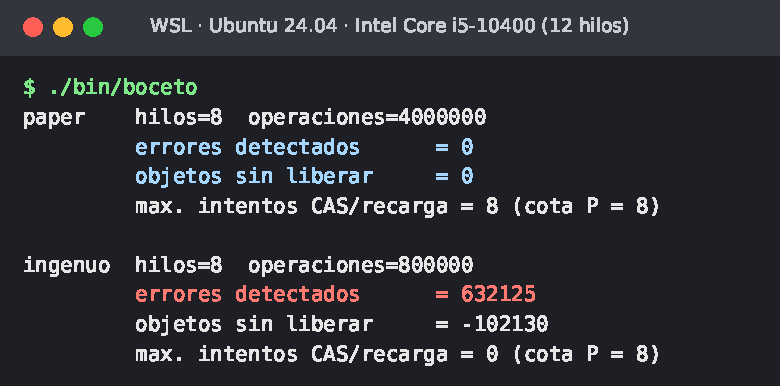
\includegraphics[width=0.8\linewidth,height=0.22\textheight,keepaspectratio]{graficos/captura_boceto.pdf}\par\smallskip
  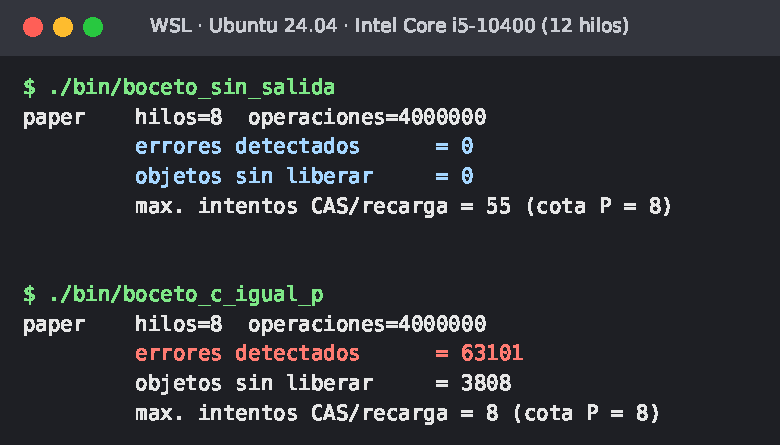
\includegraphics[width=0.98\linewidth,height=0.36\textheight,keepaspectratio]{graficos/captura_boceto_variantes.pdf}
  \begin{itemize}\footnotesize
    \item Boceto en C++, $P = 8$, $C = 16$. Paper: \textbf{0 errores}, como mucho 7 intentos ($\le P$). Ingenua: 601\,681 errores y dobles liberaciones.
    \item Sin salida temprana: 0 errores pero \textbf{38 intentos} $> P$ (no \emph{wait-free}). Con $C = P$ (rompe R-1): 50\,060 errores.
  \end{itemize}
\end{frame}

\begin{frame}{Pruebas en local (2): rendimiento con el código de los autores}
  \centering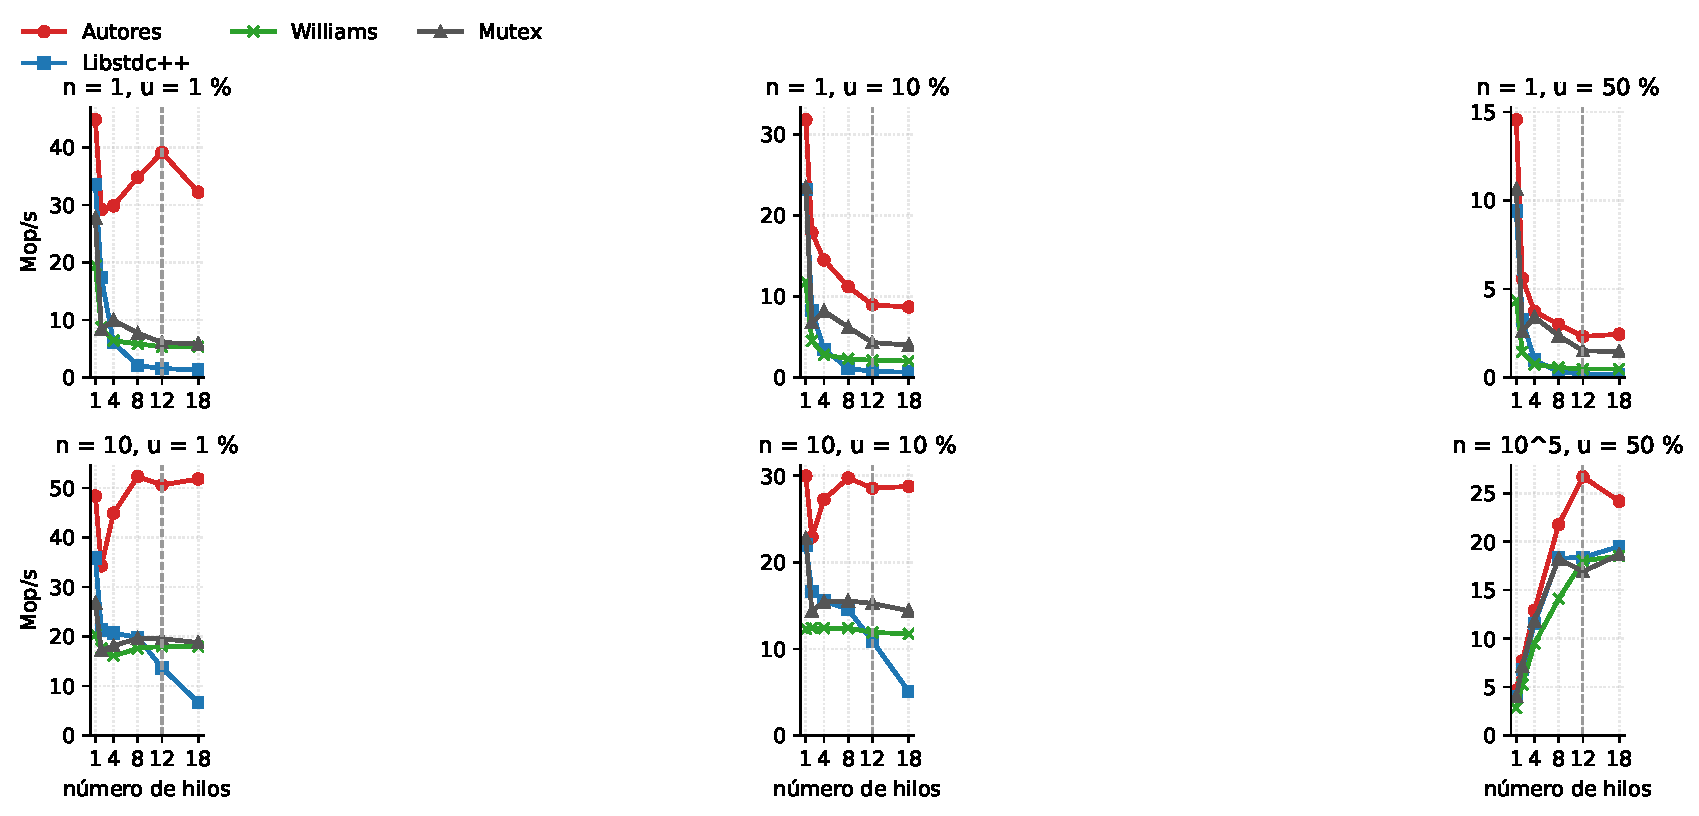
\includegraphics[width=0.8\linewidth,height=0.68\textheight,keepaspectratio]{graficos/local_rendimiento.pdf}
  \fuente{Mini-Fig. 5: pila con el código original (Autores), \texttt{atomic<shared\_ptr>} de GCC 13 (Libstdc++) y \texttt{std::mutex}. 1 s por punto; línea = 12 hilos; último panel $n = 10^5$.}
\end{frame}

\begin{frame}{Pruebas en local (3): latencia con 12 hilos}
  \centering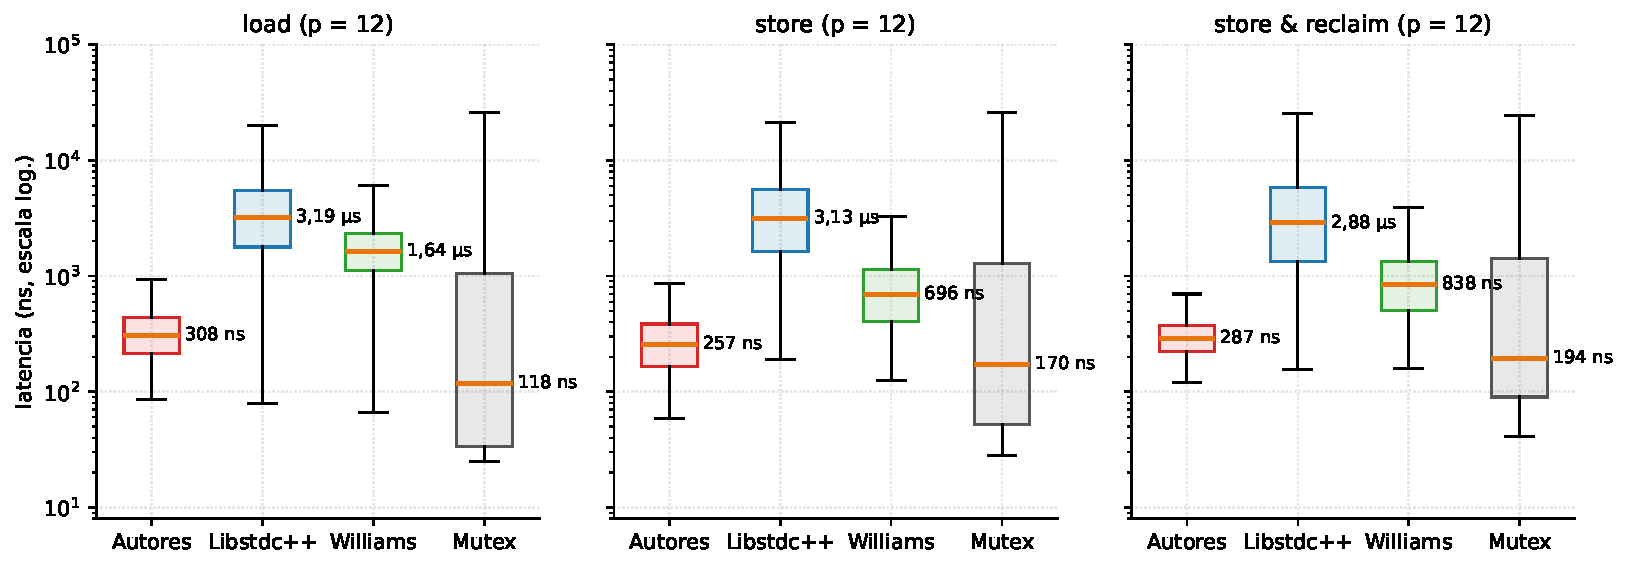
\includegraphics[width=0.8\linewidth,height=0.6\textheight,keepaspectratio]{graficos/local_latencia.pdf}
  \fuente{Mini-Fig. 6: 1 hilo mide y 11 hacen \texttt{store}; 100\,000 muestras; percentiles 1/25/50/75/99.}
  \footnotesize\par\smallskip \texttt{load}: Autores 269 ns (p99 0,83\us) · Libstdc++ 3,06\us{} (p99 16\us) · Mutex 61 ns, pero \textbf{p99 27,6\us}: la mediana engaña; la cola delata a quien espera.
\end{frame}

\begin{frame}{¿Coincide con el paper?}
  \begin{columns}[T]
    \column{0.5\textwidth}
    \textbf{\textcolor{ok}{Se reproduce}}
    \begin{itemize}\small
      \item El código de los autores: \textbf{0 errores} con AddressSanitizer; la versión ingenua cae enseguida.
      \item Con 1 hilo es la más rápida en los seis paneles.
      \item Gana con claridad a la versión con candados (GCC): con 1 pila, $u = 1$ y 12 hilos, 34,3 frente a 2,2 Mop/s.
      \item Latencia con contención: mediana y cola muy por debajo de GCC; cola mucho más corta que el mutex.
    \end{itemize}
    \column{0.47\textwidth}
    \textbf{\textcolor{acento}{Matices}}
    \begin{itemize}\small
      \item Con 1 pila y 50 \% de actualizaciones, el mutex la supera (2,9 frente a 2,2 Mop/s): el CAS \emph{lock-free} reintenta, como reconoce el paper.
      \item 12 hilos, no 144: la contención es menor y no hay sobresuscripción grande.
      \item Sin Folly, Williams ni Anderson (dependencias pesadas); WSL en Windows.
      \item Mediciones de un solo equipo y una sola ejecución: tendencias, no cifras absolutas.
    \end{itemize}
  \end{columns}
\end{frame}

\begin{frame}{Relación con el \emph{split reference count}}
  \begin{columns}[T]
    \column{0.48\textwidth}
    \begin{itemize}\small
      \item \emph{Split refcount}: un \textbf{contador local} junto al puntero, que \textbf{sube} desde 0 con cada \texttt{load} y se transfiere al objeto al cambiar el puntero.
      \item El paper cuenta lo contrario: el \textbf{peso baja} desde $C$.
    \end{itemize}
    \begin{block}{}\centering peso $= C -$ contador local\end{block}
    \small Lo nuevo no es la técnica, sino la recarga que \clave{sale si otro ya recargó}: eso la hace \emph{wait-free}.
    \column{0.49\textwidth}
    \renewcommand{\arraystretch}{1.1}\footnotesize
    \begin{tabular}{@{}lll@{}}
      \toprule
      Versión & \texttt{load} & Garantía\\
      \midrule
      Lee (2010) & FAA doble palabra & no existe en hw\\
      Williams & CAS doble anchura & \emph{lock-free}\\
      Folly & bucle CAS, $C = 8192$ & \emph{lock-free}\textsuperscript{*}\\
      \textbf{Paper} & FAA de 1 palabra & \textbf{\emph{wait-free}}\\
      \bottomrule
    \end{tabular}
    \par\smallskip{\scriptsize * Folly pasa a bloqueante con más de $C$ hilos; usa un contador de 32 bits.}
  \end{columns}
\end{frame}

\begin{frame}{Valoración crítica}
  \begin{columns}[T]
    \column{0.48\textwidth}
    \textbf{\textcolor{ok}{Fortalezas}}
    \begin{itemize}\small
      \item Sencillo: unas 30 líneas de núcleo y una demostración de una página.
      \item \texttt{load}/\texttt{store}/\texttt{swap} \emph{wait-free}, sin memoria extra, liberación inmediata (rc = 1 fiable).
      \item Lecturas de una instrucción: menor latencia y cola corta.
      \item Mejora software real (Folly, GCC) y publica su código.
    \end{itemize}
    \column{0.48\textwidth}
    \textbf{\textcolor{mal}{Límites}}
    \begin{itemize}\small
      \item CAS y \emph{aliasing} solo \emph{lock-free}.
      \item Cada lectura \textbf{escribe} en la variable compartida (no hay \emph{snapshot pointers}).
      \item Límite estricto de $P$ hilos: es de \textbf{corrección}, no de rendimiento.
      \item Depende de bits libres en el puntero (paginación de 5 niveles, ARM con PAC/MTE).
      \item No discute el orden de memoria; evalúa una estructura y una arquitectura.
    \end{itemize}
  \end{columns}
\end{frame}

\begin{frame}{Conclusiones}
  \begin{enumerate}
    \item El conteo de referencias con variables mutables puede ser \clave{wait-free sin retrasar la liberación}.
    \item La clave: un \textbf{peso prepagado} en el propio puntero; leer y apuntarse son una sola instrucción.
    \item La recarga termina en como mucho $P$ intentos gracias a R-1 ($C \ge 2P$) y R-2 (salida temprana).
    \item Funciona en la práctica: lo comprobamos en local con el código original (sin errores y mucho más rápido que la versión con candados bajo contención).
  \end{enumerate}
  \bigskip
  \textbf{Para discutir}
  \begin{itemize}\small
    \item ¿Se podría hacer el compare-and-swap \emph{wait-free} (técnicas de ayuda entre hilos) sin perder rapidez?
    \item ¿Compensaría un modo de lectura sin escritura para variables que casi nunca cambian?
  \end{itemize}
\end{frame}

{\setbeamertemplate{footline}{}
\begin{frame}[plain]
  \centering\vfill
  {\fontsize{32}{36}\selectfont\bfseries ¿Preguntas?}\par\bigskip
  {\large David · Hugo · Diego}\par\vfill
  {\small\color{gris}Código, capturas y gráficas de esta exposición: carpeta \texttt{exposicion\_paper/} (\texttt{codigo/ejecutar\_pruebas.sh})}
  \vspace*{6mm}
\end{frame}}

\expone{}
\begin{frame}{Referencias}
  \footnotesize
  \begin{itemize}
    \item I. G. de Wolff, D. Anderson, G. K. Keller y A. Seletskiy. \emph{A Fast Wait-Free Solution to Read-Reclaim Races in Reference Counting}. Euro-Par 2024, LNCS 14803, págs. 103–118. Springer. doi:10.1007/978-3-031-69583-4\_8.
    \item Código de los autores: \texttt{github.com/ivogabe/wait-free-atomic-shared-pointer} (commit 8540c58); artefacto en Zenodo, doi:10.5281/zenodo.11775182.
    \item M. Herlihy. Wait-free synchronization. \emph{ACM TOPLAS} 13(1), 1991.
    \item D. I. Bevan; P. Watson e I. Watson. Conteo de referencias ponderado. PARLE 1987.
    \item D. Detlefs, P. Martin, M. Moir y G. Steele. Lock-free reference counting. PODC 2001.
    \item H. Sundell. Wait-free reference counting and memory management. IPDPS 2005.
    \item D. Anderson, G. Blelloch e Y. Wei. Concurrent deferred reference counting with constant-time overhead. PLDI 2021.
    \item A. Williams. \emph{C++ Concurrency in Action}. Manning, 2012.
  \end{itemize}
  \fuente{Figuras y algoritmos «del paper»: reproducidos de la publicación original con fines académicos.}
\end{frame}

\begin{frame}[fragile]{Anexo: cómo reproducir las pruebas}
  \small
\begin{semiverbatim}\scriptsize
# en Linux o WSL (g++ >= 12), desde exposicion_paper/codigo
bash ejecutar_pruebas.sh        # compila y guarda todo en ../capturas
#   01 demo de los autores        02-03 AddressSanitizer (ingenua / autores)
#   04-05 boceto y variantes      06-07 rendimiento y latencia (CSV)

# simulador de intercalados (Node.js), desde exposicion_paper/simulador
node buscar.js 20000 ingenua,sinReserva

# graficas y capturas como PDF, desde exposicion_paper
python graficos/hacer_graficos.py
\end{semiverbatim}
  \smallskip
  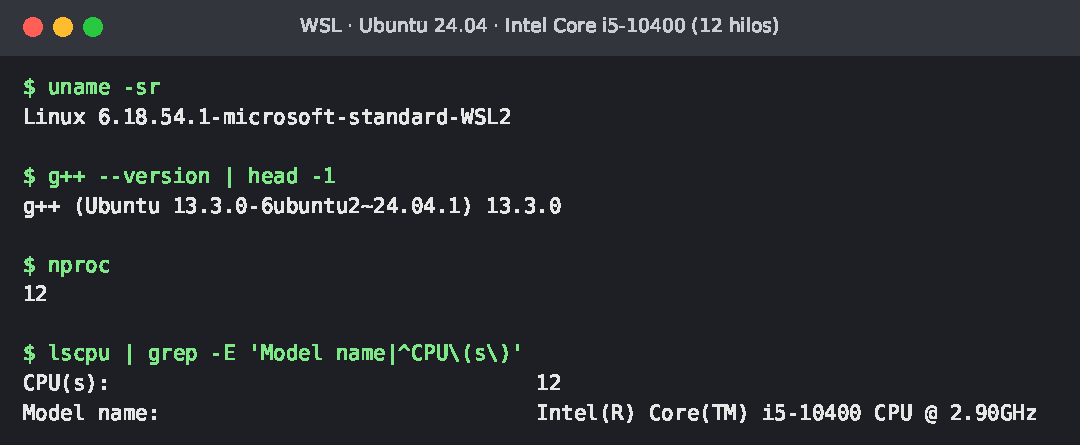
\includegraphics[width=0.5\linewidth,height=0.3\textheight,keepaspectratio]{graficos/captura_entorno.pdf}
\end{frame}

\end{document}
